\chapter{Fundamentação Teórica}\label{cap:fundamentacao}

Neste capítulo são discutidos os conceitos básicos ao entendimento deste trabalho, abrangendo processamento digital de imagens, segmentação de imagens, aprendizagem de máquina, extração de características e avaliação de desempenho dos métodos utilizados.

\section{Processamento Digital de Imagens}

Uma imagem pode ser definida por uma função bidimensional, $f(x,y)$, onde $x$ e $y$ são coordenadas espaciais de um plano, e a amplitude de $f$ para um par de coordenadas $(x,y)$ é chamada de intensidade da imagem naquele ponto. Quando $x$, $y$ e a amplitude de valores de $f$ representam quantidades finitas e discretas, podemos chamar a imagem de imagem  digital. A linha de pesquisa de processamento digital de imagens se refere ao processamento digital dessas imagens através de um computador digital \cite{gonzalez:2002}.

Uma imagem digital é composta por um número finito de elementos, cada um com um valor ($f$) e localização ($x$ e $y$) particulares. Estes elementos são chamados de elementos da imagem ou \textit{pixels}, do inglês \textit{picture elements}.

Ainda de acordo com \citeonline{gonzalez:2002}, o interesse em processamento digital de imagens advém de duas principais áreas de aplicação: melhoramento de informações pictóricas para interpretação humana; e processamento de imagens para armazenamento e transmissão de dados, e representação para percepção de máquinas autônomas. 

Em muitos problemas, como o de interpretação de imagens por uma máquina, é comum que algum processo de segmentação seja realizado, e as imagens sejam divididas em regiões para processamento posterior.

\subsection{Segmentação de Imagens}

O processo de segmentação subdivide uma imagem em suas várias regiões ou objetos. O nível em que a subdivisão é feita depende do problema a ser resolvido, ou seja, a segmentação deve parar quando os objetos de interesse de uma aplicação forem isolados. Por exemplo, na inspeção automática de uma linha de montagem de produtos eletrônicos, o interesse reside em analisar imagens dos produtos com o objetivo de determinar a presença ou ausência de anomalias específicas, como componentes faltando ou conexões quebradas. Não há sentido em continuar segmentando além do nível de detalhes necessário para a identificação destes elementos.

Segmentação de imagens é um dos problemas mais difíceis em processamento digital de imagens \cite{gonzalez:2002}. Algoritmos de segmentação geralmente se baseiam em uma das duas propriedades básicas de valores de intensidade dos pixels: descontinuidade e similaridade. Na primeira propriedade, a abordagem é particionar a imagem baseando-se em mudanças abruptas na intensidade dos pixels, como as bordas. A segunda categoria se baseia no particionamento de uma imagem em regiões que são similares de acordo com um critério em particular, que pode ser coloração, textura, entre outros.

Neste trabalho, conforme será descrito no capítulo \ref{cap:metodologia}, testamos uma série de atributos para determinar a melhor forma de segmentar as regiões das imagens aéreas da floresta amazônica, como uma das etapas da pesquisa de detecção de anomalias. Muitas vezes, técnicas de segmentação de imagens não são suficientes para isolar ou detectar componentes específicos na coleção de imagens. Trabalhos recentes têm utilizado, com frequência, algoritmos de aprendizagem de máquina para resolver este problema.


\section{Aprendizagem de máquina e reconhecimento de padrões}

Conforme \citeonline{alpaydin:2010}, aprendizagem de máquina é uma área da inteligência artificial que estuda métodos computacionais, a fim de obter um determinado conhecimento específico através de experiências. A aplicação prática de aprendizado de máquina inclui o processamento de linguagem natural, diagnósticos médicos, detecção de intrusos, entre outros. Um sistema de aprendizado tem a função de analisar informações e generalizá-las, para a extração de novos conhecimentos.

Segundo \citeonline{russell:2010}, os tipos de aprendizagem podem ser classificados de acordo com o tipo de \textit{feedback} que recebem do ambiente:

\begin{itemize}
    \item Aprendizagem não-supervisionada: o agente aprende padrões na entrada, embora não seja fornecido nenhum \textit{feedback} explícito. A tarefa mais comum de aprendizagem não-supervisionada é o agrupamento, ou seja, a detecção de grupos de exemplos de entrada potencialmente úteis.
    \item Aprendizagem por reforço: também conhecida como aprendizagem semi-supervisionada. O agente aprende a partir de uma série de reforços - recompensas ou punições.
    \item Aprendizagem supervisionada: o agente observa alguns exemplos de pares de entrada e saída, e aprende uma função que faz o mapeamento da entrada para a saída.
\end{itemize}

Os problemas de aprendizagem podem ainda ser divididos de acordo com o tipo de saída que demandam:

\begin{itemize}
	\item Problemas de classificação: quando a saída esperada para o problema é uma classe ou categoria, ou seja, um valor discreto;
	\item Problemas de regressão: quando a saída esperada para o problema é um valor numérico, normalmente contínuo.
\end{itemize}

Um problema de classificação, ou seja, um problema em que o objetivo é atribuir corretamente classes discretas (rótulos) aos exemplos de dados, consiste na determinação de regras e posterior classificação desses exemplos. Este conjunto de regras é criado por um classificador, que recebe como entrada um vetor de características e oferece como saída uma classe resultante para a instância que as características descrevem, conforme pode ser visto na figura \ref{fig:classificador}.

\begin{figure}[h!]
  \centering
  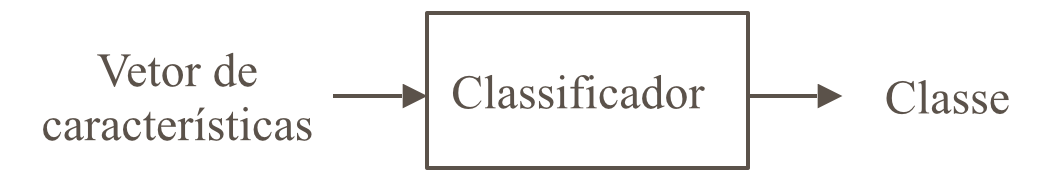
\includegraphics[width=0.7\textwidth]{imgs/classificador}
  \caption{Representação de classificador como uma função de bloco}
  \label{fig:classificador}
\end{figure}

Os tipos de classificadores utilizados neste trabalho serão discutidos com mais detalhes na seção \ref{sec:classificacao}.

Para composição do modelo de aprendizagem, uma base de dados de treinamento é utilizada. Esta base deve possuir uma quantidade significativa e com boa representatividade das classes envolvidas no problema. Normalmente se usa uma parte da base de dados de treinamento para validação do modelo de aprendizado (validação cruzada) ou mesmo uma base de dados diferente (base de testes ou validação), para que indicadores de qualidade do modelo possam ser avaliados. A seção \ref{sec:avaliacao} discorre sobre os métodos de avaliação utilizados neste trabalho.

Técnicas de aprendizagem de máquina podem ser utilizadas para encontrar padrões em diversos domínios, inclusive em imagens. É neste ponto que a linha de pesquisa de aprendizagem de máquina, advinda da área de inteligência artificial, se encontra com a linha de pesquisa de reconhecimento de padrões, advinda da área de processamento de sinais. Segundo \citeonline{jain:1989}, o fluxo padrão para soluções de reconhecimento de padrões consiste em três etapas:

\begin{enumerate}
    \item Filtragem e pré-processamento da entrada;
    \item Extração e seleção de características;
    \item Classificação.
\end{enumerate}


\subsection{Filtragem e Pré-processamento}

A etapa de filtragem e pré-processamento é responsável pela escolha e montagem da base de dados que será usada no processo de aprendizagem. A base deve conter uma quantidade significativa de exemplos de todas as classes envolvidas no problema.

Em aprendizado relacionado a imagens, essa etapa é comumente a responsável por normalizar e salientar as características desejadas nas amostras (realce de imagens, filtragem, etc). Exemplos irrelevantes, distorcidos ou repetidos também são eliminados durante a filtragem. O objetivo principal desta etapa é preparar a base de dados para as etapas seguintes.


\subsection{Extração de Características}

A extração de características é feita selecionando os atributos oriundos dos dados (imagens, no trabalho em questão), a fim de encontrar as características úteis para o processo de reconhecimento. Essa etapa é crítica ao sucesso do aprendizado, uma vez que bons algoritmos de aprendizado só obtêm êxito com um bom conjunto de características relevantes ao problema.

Em projetos que envolvem classificação de imagens, uma gama de atributos pode ser extraída, e podem ser descritos pelo nível da informação que representam. Nesta etapa há uma forte contribuição da linha de pesquisa de processamento digital de imagens \cite{gonzalez:2002}, que descreve filtragens, transformações e outras técnicas capazes de extrair informações sobre uma imagem ou pedaços dela.

Segundo \citeonline{nixon:2008}, informações de baixo-nível como bordas, histogramas de intensidade e coloração, são úteis para o reconhecimento de padrões em imagens, assim como características de níveis mais altos, como texturas, transformadas de Hough e extração de regiões conectadas.

O produto desta etapa é a representação de cada exemplo da base de dados em um vetor de características, de forma que possa ser usado por um ou mais classificadores em uma etapa posterior.


\subsection{Classificação}\label{sec:classificacao}

Nesta etapa, todas as amostras de treinamento são classificadas e um modelo de aprendizado é gerado. Posteriormente ao processo de aprendizado, é nesta mesma etapa que as amostras não classificadas receberão uma classe dentre as envolvidas no problema. É neste momento que podemos comparar o desempenho de diferentes algoritmos de aprendizado para o conjunto de características escolhido para representar o problema.

Pode-se também usar múltiplos classificadores, ao invés de apenas um. Esta abordagem é chamada de sistemas com múltiplos classificadores (do inglês \textit{multiple classifier systems}), os quais podem ser compostos por classificadores do mesmo tipo (denominado \textit{Ensemble} de classificadores) ou de diferentes tipos. Existe uma grande variedade de algoritmos de aprendizagem de máquina propostos na literatura. Alguns dos mais utilizados são: classificadores estatísticos, redes neurais artificiais, árvores de decisão, máquinas de vetores de suporte (SVM), k vizinhos mais próximos (KNN), etc \cite{jain:1989}.

Amplamente utilizadas em algoritmos de classificação, as árvores de decisão são representações simples do conhecimento e um meio eficiente de construir classificadores que predizem classes baseadas nos valores de atributos de um conjunto de dados. As árvores de decisão consistem de nodos que representam os atributos; de arcos, provenientes destes nodos e que recebem os valores possíveis para estes atributos; e de nodos folha, que representam as diferentes classes de um conjunto de treinamento. Classificação, neste caso, é a construção de uma estrutura de árvore, que pode ser usada para classificar corretamente todos os objetos do conjunto de dados da entrada.

A partir de uma árvore de decisão é possível derivar regras. As regras são escritas considerando o trajeto do nodo raiz até uma folha da árvore. Estes dois métodos são geralmente utilizados em conjunto. Devido ao fato das árvores de decisão tenderem a crescer muito, de acordo com algumas aplicações, elas são muitas vezes substituídas pelas regras. Isto acontece em virtude das regras poderem ser facilmente modularizadas. Uma regra pode ser compreendida sem que haja a necessidade de se referenciar outras regras.

Uma árvore de decisão tem a função de particionar recursivamente um conjunto de treinamento, até que cada subconjunto obtido deste particionamento contenha casos de uma única classe. Para atingir esta meta, a técnica de árvores de decisão examina e compara a distribuição de classes durante a construção da árvore. O resultado obtido, após a construção de uma árvore de decisão, são dados organizados de maneira compacta, que são utilizados para classificar novos casos. A árvore de decisão não presume nenhum modelo estatístico a priori, sendo a divisão do espaço de atributos feita de acordo com as amostras provenientes do treinamento.

O algoritmo KNN (K-Nearest Neighbours, ou K vizinhos mais próximos) \cite{cover:1967} é um método de classificação baseado na proximidade de amostras de treino no espaço de características. É considerado um dos mais simples algoritmos de aprendizagem de máquina.

O processo de treinamento para esse algoritmo consiste em armazenar o vetor de característica e rótulos (classes) de cada amostra de treinamento em um espaço n-dimensional, onde n é o número de características de cada amostra. No processo de classificação de amostras não-rotuladas, a amostra é simplesmente projetada no espaço e é classificada de acordo com as k amostras mais próximas.

Quando k = 1, a amostra é simplesmente classificada de acordo com o rótulo de seu vizinho mais próximo no espaço de características. Quando k é maior que 1, a classificação se dá por um esquema de votação, onde a classe com as amostras vizinhas mais numerosas é considerada como a classe da amostra. Por essa razão, em problemas bi-classe como o apresentado neste artigo devem possuir um k ímpar, para evitar empates. Em problemas multi-classe, ou seja, com mais de duas classes possíveis, empates podem acontecer mesmo considerando um número ímpar de vizinhos, de maneira que uma forma de desempate deve ser definida na implementação do algoritmo.

Diversas formas de calcular a distância entre duas amostras $a$ e $b$ em um espaço n-dimensional podem ser utilizadas no kNN, dentre elas a distância Euclidiana, representada pela fórmula \ref{eq:euclides}, onde $n$ é o número de dimensões.

\begin{equation}
	\displaystyle d(a,b) = ||a - b|| = \sqrt{(a - b)*(a -b)} =
	\displaystyle \sqrt{\sum_{i=1}^{n}(a_i - b_i)^2}
\label{eq:euclides}
\end{equation}

As máquinas de vetores de suporte, ou SVM (\textit{Support Vector Machines}) são classificadores baseados na teoria de aprendizagem estatística proposta por \cite{vapnik:1995}. A teoria é baseada em uma forte fundamentação matemática para estimação de dependências e previsão do aprendizado a partir de conjuntos de dados finitos. 

Um modelo SVM é a representação das amostras como pontos em um espaço n-dimensional (onde n é o tamanho do vetor de características) de tal forma que as amostras de diferentes classes sejam divididas por um plano de separação que maximiza a distância entre essas classes. Isso se deve ao fato de que o plano de separação possui a maior distância possível às amostras mais próximas entre as classes, o que ajuda a diminuir o erro de generalização (\textit{over-fitting}) do classificador.

A principal vantagem do classificador SVM é seu bom desempenho em conjuntos de dados que possuem muitos atributos, mesmo quando há poucas amostras de treino. No entanto, suas desvantagens são a baixa velocidade e alto consumo de recursos durante as fases de treinamento, assim como a complexidade de parametrização de suas funções \textit{kernel}. As amostras de teste são classificadas ao serem posicionadas no espaço de características e avaliadas em que lado da superfície de separação elas se encontram, como mostrado na figura \ref{fig:svm}.

\begin{figure}[h!]
  \centering
  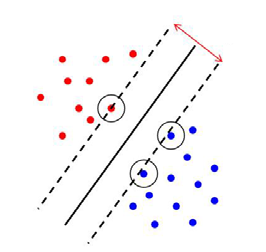
\includegraphics[scale=0.5]{imgs/svm}
  \caption[Máquina de vetores de suporte]{Amostras em um espaço bidimensional (pontos coloridos) separadas por um hiperplano apoiado por vetores de suporte (setas vermelhas), maximizando a distância entre as amostras mais próximas entre as classes (pontos circulados)}
  \label{fig:svm}
\end{figure}

O algoritmo \textit{Random Forest}, introduzido por \citeonline{breiman:2001} , é um \textit{ensemble} de classificadores de árvore de decisão. Na fase de treinamento, um número determinado de árvores é gerado utilizando um subconjunto pseudo-aleatório do vetor de característica completo utilizado no problema. Tanto o número de árvores quanto a quantidade de atributos utilizados por cada árvore pode ser determinado pelo usuário do algoritmo.

Uma vez que a base de treinamento foi utilizada para gerar os modelos das árvores de decisão, estes mesmo modelos podem ser utilizados para classificar novas amostras do problema. Preferencialmente todas as árvores geradas são envolvidas na classificação, cada uma chegando à sua própria conclusão sobre a classe da amostra apresentada. Cada árvore tem um ``voto'', que é contabilizado para a definição da classe mais votada, que é então escolhida como a classe da amostra. Esta técnica de soma de votos é conhecida como \textit{polling}.

A principal vantagem deste algoritmo é a eliminação de \textit{overfitting}, problema bastante comum quando se utiliza árvores de decisão de forma tradicional. Uma exposição mais detalhada acerca de \textit{overfitting} é feita na seção \ref{sec:avaliacao}.

O trabalho de \citeonline{breiman:2001} ainda afirma que a taxa de erro de um modelo de aprendizado criado com \textit{Random Forest} está relacionada a dois fatores: a correlação entre quaisquer duas árvores geradas no modelo e a ``força'' de cada árvore gerada, ou seja, o quão precisa ela é em relação ao modelo geral. À medida que a correlação entre árvores cresce, também cresce a taxa de erro do modelo final. Quanto menor for a taxa de erro de uma árvore individual, mais ``forte'' é considerado o classificador, e por consequência, mais baixo é a taxa de erro do modelo.

Reduzir o número de variáveis do vetor de características a ser utilizado em cada árvore reduz a correlação entre árvores e também reduz a ``força''da árvore. Incrementar este número de variáveis incrementa a correlação e a ``força'' da árvore. A parametrização do algoritmo deve se preocupar em encontrar o número de variáveis do vetor de característica que melhor minimize a correlação e maximize a ``força'' das árvores do modelo.

Tanto durante o desenvolvimento de uma solução, quanto após sua execução em ambiente de produção, é preciso aferir e quantificar o desempenho da técnica desenvolvida ou utilizada, conforme discutido na próxima seção.

\section{Avaliação}\label{sec:avaliacao}

Avaliar o desempenho de uma técnica de aprendizagem de máquina é útil para determinar a qualidade do modelo criado, aferir se o modelo continua adequado e inspecionar se os atributos escolhidos são relevantes para a classificação das amostras.

Comumente, o percentual de acerto obtido na classificação das amostras é um importante parâmetro para medir o desempenho do modelo. Este parâmetro é conhecido como acurácia ou taxa de reconhecimento. O oposto da acurácia é conhecido como taxa de erro.

De grande importância também é a composição da matriz de confusão (tabela \ref{tab:matrixConfusao}). Nela pode-se avaliar como um modelo está se comportando em termos de falsos positivos (Um exemplo é classificado como pertencente à classe C, mas não é) e falsos negativos (um exemplo é atribuído a outra classe, mas deveria ser da classe C). A principal função desta matriz é dar possibilidade de pensar sobre o custo dos erros, ou seja, mesmo que a taxa de acerto para o problema seja alta, uma ou mais classes do problema pode ter uma taxa de acerto bem abaixo do esperado.

\begin{table}[h]
  \centering
  \begin{tabular}{cccc}
  \multicolumn{2}{c}{\textbf{Resultado obtido}}                  &                               &                                              \\ \cline{1-2}
  \multicolumn{1}{|c|}{Classe A} & \multicolumn{1}{c|}{Classe B} &                               &                                              \\ \cline{1-3}
  \multicolumn{1}{|c|}{Verdadeiro positivo}       & \multicolumn{1}{c|}{Falso negativo}       & \multicolumn{1}{c|}{Classe A} & \multirow{2}{*}{\textbf{Resultado esperado}} \\ \cline{1-3}
  \multicolumn{1}{|c|}{Falso positivo}       & \multicolumn{1}{c|}{Verdadeiro negativo}       & \multicolumn{1}{c|}{Classe B} &                                              \\ \cline{1-3}
  \end{tabular}
  \caption{Modelo de matriz de confusão.}
  \label{tab:matrixConfusao}
\end{table}

Alguns valores podem ser obtidos através desta matriz. A própria acurácia do modelo pode ser obtida com a equação \ref{eq:acuracia}, onde TP representa o número de verdadeiros positivos, FP representa os falsos positivos, FN representa os falsos negativos e TN representa os verdadeiros negativos.

\begin{equation}
  Acurácia = \frac{TP+TN}{TP+FP+TN+FN}
\label{eq:acuracia}
\end{equation}

Ainda é possível obter a precisão e a revocação. A precisão é o número de elementos relevantes recuperados dividido pelo número total de elementos recuperados (equação \ref{eq:precisao}) enquanto a revocação é definida como o número de elementos relevantes recuperados dividido pelo número total de elementos relevantes existentes, que deveriam ter sido recuperados (equação \ref{eq:revocacao}).

\begin{equation}
  Precisão = \frac{TP}{TP+FP}
\label{eq:precisao}
\end{equation}


\begin{equation}
  Revocação = \frac{TP}{TP+FN}
\label{eq:revocacao}
\end{equation}

Apesar de que a maximização da acurácia seja desejável para o ajuste de um algoritmo de aprendizado, é importante haver cuidado com o o sobreajuste (\textit{overfitting}) que pode ser gerado a partir disto. O \textit{overfitting} é o termo utilizado quando o modelo criado se ajusta em excesso às amostras de treinamento, tendo altas taxas de acurácia para esta base, mas falhando em classificar com boa taxa de acurácia as demais amostras de teste ou amostras reais.

Em resumo, o problema é ter um modelo que possui bom desempenho na etapa de treinamento mas não é uma boa representação das amostras reais. A figura \ref{fig:overfitting} exemplifica um modelo de classificação generalista (linha preta) e um modelo que sofre de \textit{overfitting} (linha verde).

\begin{figure}[h!]
  \centering
  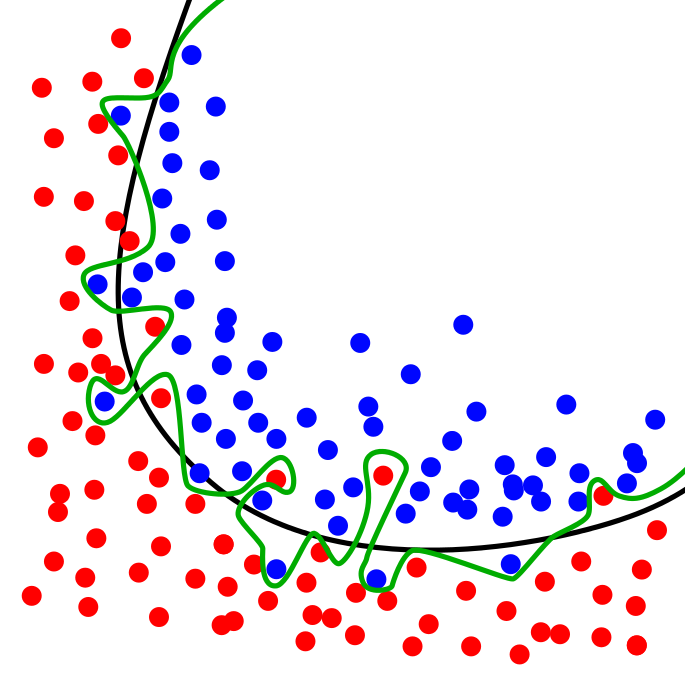
\includegraphics[scale=0.3]{imgs/overfitting}
  \caption{Modelo de aprendizado em um problema de duas classes, a linha preta indica uma função mais generalista, enquanto a linha verde representa uma função mais adequada às amostras de treinamento, mas que provavelmente sofre de \textit{overfitting.}}
  \label{fig:overfitting}
\end{figure}

Para detectar problemas de \textit{overfitting}, pode-se testar o modelo em diversas outras bases de amostra, medindo a variância da acurácia entre estas bases. Uma alta variância indica que o modelo não é genérico o suficiente, apontando para um provável caso de \textit{overfitting}.

Uma vez que a fundamentação teórica necessária foi coberta, é necessário fazer um levantamento na literatura pelos trabalhos considerados estado da arte em suas respectivas áreas. O capítulo a seguir trata deste levantamento.